\chapter{绪论:初识机器学习}

\begin{center}
学而不思则罔,思而不学则怠!
\end{center}

\begin{flushright}
---孔子    
\end{flushright}

\section{欢迎参加机器学习课程}
机器学习是最激动人心的技术。在很多方面都使用了机器学习技术。机器学习主要的应用方向:
\begin{itemize}
\itemsep=3pt
\parskip=0pt
\item 数据挖掘
\item 在无法手动编写的程序中的应用
\item 在私人定制程序中的应用
\end{itemize} 

\section{什么是机器学习}

本节课程的主要内容有两个:
\begin{enumerate}[1)]
\item 机器学习的定义
\begin{newdef}[Arthur Samuel]
\large 在没有明确设置的情况下使计算机具有学习能力的研究领域。
\end{newdef}

\begin{newdef}[Tom Mitchell]
\large 对于某类任务T和性能度量P,如果一个计算机程序在T上以P衡量的
性能随着经验E而自我完善,那么我们称这个计算机程序在从经验E学习。\cite{MachineLearning}
\end{newdef}
\item 在什么情况下使用机器学习

常用机器学习算法一般可以分为两类:
\begin{itemize}
\item 监督学习{\color{red} ---教会计算机做某件事情。}
\item 无监督学习{\color{red} ---让计算机自己学习。}
\end{itemize}

\end{enumerate}

\section{监督学习}

\subsection{回归问题}
使用波特兰房屋价格的例子来说明监督学习,采集的数据如下图1.1所示,横轴表示的是平方英尺数,纵轴是不同房子的价格,单位是千美元。

\begin{figure}[!hbtp]
\centering
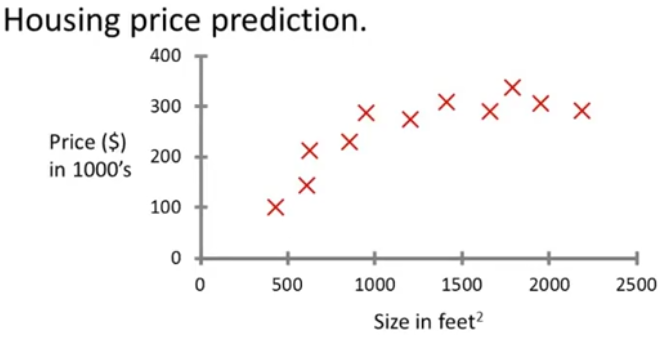
\includegraphics[width=0.8\textwidth]{room_price.png}
\caption{Room Price\label{figur:root_price}}
\end{figure}

假设你的朋友有一栋750平方英尺的房子,他想要卖掉房子,需要预测一下能够卖多少钱,此时学习算法能够有什么帮助呢?
根据数据画一条直线,或者说一条直线拟合数据,如图1.2所示,由此看房子大约可以卖15万美元。
\begin{figure}[H]
\centering
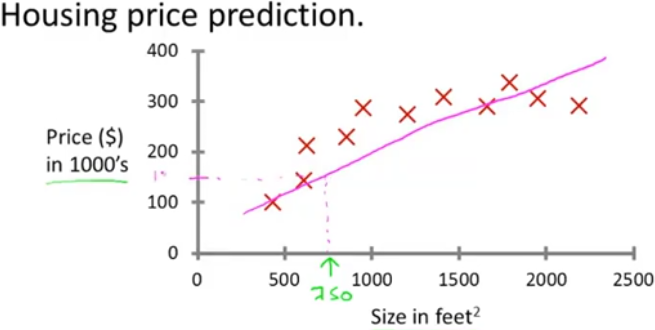
\includegraphics[width=0.8\textwidth]{room_price_1.png}
\caption{Room Price fitting straight\label{figur:root_price_1}}
\end{figure}

当然这并不是唯一能使用的学习算法,例如除了使用一条直线来拟合之外,还可以采用二阶函数或者二阶多项式来拟合,这样可能会更好,如图1.3
所示,此时你再做预测,看上去房子可以卖出接近20万美元。
\begin{figure}[!hbtp]
\centering
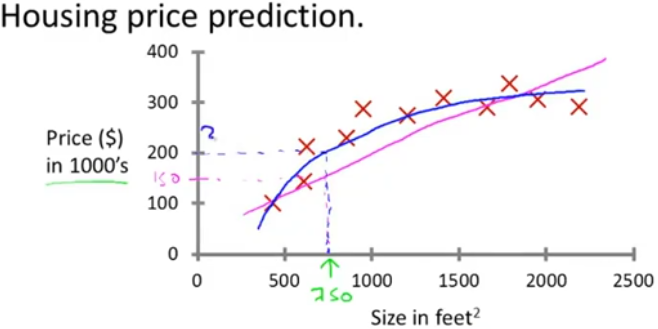
\includegraphics[width=0.8\textwidth]{room_price_2.png}
\caption{Room Price Second Derivative\label{figur:root_price_2}}
\end{figure}

而我们需要讨论的一件事就是如何选择如何决定,是采用直线来拟合数据,还是采用二阶函数来拟合,
当然无论采用哪个模型都不会让你的朋友房子的价格卖的更好,但这是一个学习算法很好的例子,这
是一个监督学习算法的例子。

监督学习是指我们给算法一个数据集,其中包含了正确答案,也就是说我们给他一个房价数据集,在
这个数据集中的每个样本,我们都给出正确的价格,即这个房子实际卖价,算法的目的就是给出更多
的正确答案,例如为你朋友想要卖掉的这所新房子给出估价,用更专业的术语来说,它也被称为回归问题。
这里的回归问题指的是我们想要预测连续的数值输出,也就是价格,技术上而言价格能够被圆整到分,
因此是一个离散值,但通常我们认为房价是一个实数标量或是连续值,回归问题是我们设法预测连续值
的属性。

\subsection{分类问题}
这里有另一个监督学习的例子,设法预测乳腺癌是恶性还是良性,假设某人发现了一个乳腺肿瘤即乳房上的肿块,需要预测是良性肿瘤还是恶性肿瘤,
我们先来看看搜集的数据集如图1.4所示,横轴是肿瘤的尺寸,纵轴画了1或者0来代表是或者否,即看到的肿瘤是否是恶性的,恶性的对应1,良性的
对应0。
\begin{figure}[H]
\centering
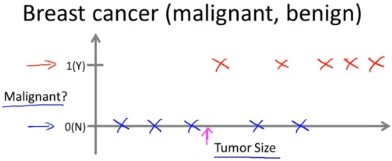
\includegraphics[width=0.8\textwidth]{tumor_prediction.jpg}
\caption{Tumor Prediction\label{figur:tumor_prediction}}
\end{figure}

假设有一个朋友不幸的患了乳腺肿瘤,她的肿块尺寸在图1.4红色箭头所指向的位置,机器学习的问题就是你能否估计出肿瘤是良性的还是恶性
的概率,用更专业的术语来说,这就是一个分类问题,分类是指我们设法预测一个离散值输出,0或1恶性或良性,其实在分类问题中有时候也有两个以
上的可能的输出值,在实际的例子中就是可能有三种类型的乳腺癌,因此可能要设法预测离散值0、1、2或3,即没有癌症,或者癌症1,癌症2,癌症3。
在分类问题中有另外一种方法来绘制这些数据,如图1.5所示,将所有数据都对应下来。
\begin{figure}[H]
\centering
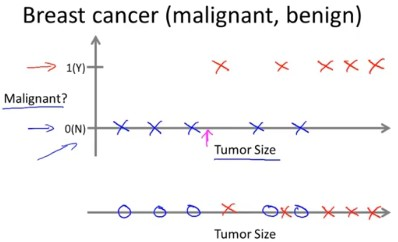
\includegraphics[width=0.8\textwidth]{tumor_prediction_1.jpg}
\caption{Tumor Prediction figure\label{figur:tumor_prediction_1}}
\end{figure}

在其它的机器学习问题中我们会有多个特征,多个属性,这里有个例子,假设我们不仅知道肿瘤的大小,还知道病人的年纪,在这种情况下数据集会如
图1.6所示,假设有个朋友不幸的得了肿瘤,他肿瘤位于红色点的位置,我们可以用一条线来分离这两类肿瘤,此时机器算法可以判断该朋友的肿瘤位
于良性区域。
\begin{figure}[hbtp]
\centering
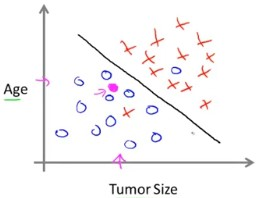
\includegraphics[width=0.8\textwidth]{tumor_area.jpg}
\caption{Tumor Area figure\label{figur:tumor_area}}
\end{figure}
在其它的机器学习算法中,往往会有更多的特征,我的朋友研究了这样的问题,他们实际上使用了别的特征,例如肿块的厚度,肿瘤细胞形状的均匀性,
以及其它特征,在本课程中我们将看到的最有趣的学习算法是一个不仅仅能处理两个到三个或五个特征,而是能处理无穷多个特征的算法,在本节中只
提到了五个不同的特征,但是对于某些机器学习问题,需要处理无穷多个特征,机器学习算法需要用到无穷多的属性,但是计算机明显是不
能存储无穷多的特征,因为计算机可能会溢出,以支持向量机为例子,假设我写下无穷长的列表,无限长的特征,其实我们能设计一个算法来处理这种
情况。
\begin{figure}[H]
\centering
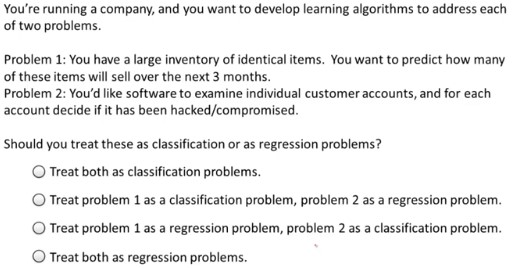
\includegraphics[width=0.8\textwidth]{question_01.jpg}
\caption{Question01\label{figur:question_01}}
\end{figure}
概括一下在这节课上我们讨论了监督学习,想法是在监督学习中,对于数据集中的每个样本,我们想要算法预测,并得出的“正确答案”,像房子的价格
或肿瘤是恶性的还是良性的,我们也讨论了回归问题,回归是指我们的目标,是预测一个连续值输出,我们还讨论了分类问题,其目的是预测离散值输
出,最后提一个小问题,问题如图1.7所示。

\section{无监督学习}
无监督学习告诉你更多哦。
\section{问题}
学习之后就要思考问题。